\documentclass[times, utf8, seminar]{fit}

%\batchmode
%\usepackage{booktabs}
\usepackage{listings}
\usepackage{longtable}
\usepackage{xcolor}
\usepackage{float}
\usepackage{enumitem}
\usepackage{hyperref}
\usepackage{enumerate}
\usepackage{graphicx}
\usepackage{etoolbox}
\usepackage{datetime}
\usepackage{needspace}
\usepackage{titlesec}
%\titleformat{\chapter}[display]{\normalfont\huge\bfseries}{\chaptertitlename\ \thechapter}{20pt}{\Huge}

\begin{document}
\widowpenalty=300
\clubpenalty=300

% this alters "before" spacing (the second length argument) to 0
%\titlespacing*{\chapter}{0pt}{0pt}{40pt}

% this changes "before" spacing back to its default of 50pt
%\titlespacing*{\chapter}{0pt}{50pt}{40pt}}

%\titlespacing*{\chapter}{0pt}{-50pt}{18pt}
%\titleformat{\chapter}[display]{\normalfont\huge\bfseries}{\chaptertitlename\ \thechapter}{20pt}{\Huge}

\title{Open source software in Bosnia and Herzegovina}

\author{Ernad Husremović}
\brindex{DL 2792}
\verzija {0.9.5}

\mentor{Iris Memić}

\maketitle

\tableofcontents

%\listoftables
%\listoffigures
\newpage

% abstract begin
%\begin{abstract}
%
%To be done 
%
%\keywords{open source software, OSS, Bosna i Hercegovina}
%\end{abstract}

% abstract end

\chapter{Introduction}

\section{Open source software}

Open source software (OSS) refers to the software that is released with source code. The core philosophy of open source is sharing.

OSS Community is the place where the sharing takes place.

OSS projects are typically a collaborative effort in which programmers create and share the code within the community.

\subsection{Open source definition by Bruce Perens}
Bruce Perens was the first person who announced "Open Source" to the world in 1998, and is the creator of the Open Source Definition\footnote{\url{http://www.opensource.org/docs/osd}}, the manifesto of the Open Source movement and the rules required for a software license to be considered "Open Source"\citep{web:perens}. Today, Perens works as the leader in the Open Source and Free Software community. He advises many large companies and several national governments on issues related to Open Source. Perens' main policy areas regarding Open Source are:

\begin{center}
\emph{\large{Freedom to create, distribute, and use open source software (OSS).}}
\end{center}


\subsection{Open source vs. Free Software}

In his Open Source work, Perens is standing on the shoulders of giants: in particular \emph{Richard Stallman}, founder of the Free Software movement\footnote{\url{http://www.gnu.org/philosophy/free-software-intro.html}} in the early 1980’s. Perens positions Open Source as a different way of talking about Free Software, intended for a different audience - business people and those who would be more receptive to an economic and pragmatic argument than to Stallman's focus on Freedom\citep{web:perens}.

Perens believes that Open Source and Free Software belong to the same movement rather than two conflicting ones. Perens believes that promotion of Open Source should not deprecate Stallman or his philosophy.

Stallman himself understands, but does not entirely accept Perens' slant on using the language of Open Source to promote Free Software. This is Stallman's statement:

\begin{quotation}
\emph{Free software and Open Source seem quite similar, if you look only at their software development practices. At the philosophical level, the difference is extreme. The Free Software Movement is a social movement for computer users' freedom. The Open Source philosophy cites practical, economic benefits. A deeper difference cannot be imagined.}
\end{quotation}

Despite their differences, Perens and Stallman maintain a good relationship and work together frequently.

\section{The social aspect of OSS}

Open source is a phenomenon of today's IT industry. It has changed the paradigm of software development. Many development practices which were firstly promoted with OSS development, are today's universal praxis. The social aspect is doubtless one of the most important factors of OSS.

\subsection{Linus's Law}

Linus's Law as described by Raymond is a claim about software development, named in honor of Linus Torvalds and formulated by Raymond in his essay and book ``The Cathedral and the Bazaar''\citep{bazaar}. The law states:

\begin{center}
\emph{\large{Given enough eyeballs, all bugs are shallow.}}
\end{center}

More formally: "Given a large enough beta-tester and co-developer base, almost every problem will be characterized quickly and the fix will be obvious to someone." Presenting the code to multiple developers with the purpose of reaching consensus about its acceptance is a simple form of software reviewing. Researchers and practitioners have repeatedly shown the effectiveness of the reviewing process in finding bugs and security issues, and also that reviews may be more efficient than testing\footnote{\url{http://en.wikipedia.org/wiki/Linus'\_Law}}.

\section{Open source licences}

Software license determines constraints on software usage and redistribution. Two main categories of licenses are "proprietary" and "free and open source" (FOSS) licenses.

Later, FOSS licenses fall in two main categories:
\begin{itemize}
  \item copyleft licenses
  \item permisive licenses 
\end{itemize} 

Copyleft licenses are focused on preserving freedom to study, modify and use software by all users. Consequently they force authors to release modifications under the same terms. It is the reason they are sometimes referred to as "viral licenses".

Permissive licenses have minimal requirements on preserving openness to subsequent users. The main characteristic of permissive licenses is the possibility to take the source code and merge with closed source software. The author of modifications decides whether they will be released as closed software or as open source software. The possibility to mix closed and open source code tags permissive licenses as „business friendly".

GNU General Public License\footnote{\url{http://www.gnu.org/copyleft/gpl.html}} is the main representant of copyleft licenses.

MIT\footnote{\url{http://www.opensource.org/licenses/mit-license.html}} and BSD licenses\footnote{\url{http://www.opensource.org/licenses/BSD-3-Clause/}} are the most popular permissive licenses.

\section{OSS business models}

There are many business models based on OSS\footnote{\url{http://www.opensourcestrategies.org/}}. Two main categories are: 
\begin{itemize}
  \item service based
  \item open core
\end{itemize}

Service based OSS business offers its expertise and support to its customers. The software itself is free and open source and isn't the subject of business offer.

"Open core" model offers basic functionalities as open source and advanced (enterprise) features as closed source.

There is lot criticism on the "open core" model. The opponents argue that "open core" is much like a trial versions of closed software.

The choice of specific model is highly correlated by the class of the software.  For example, "open core" model is largely applied among ERP\footnote{Enterprise Resource Planning} software.  

\section{OSS projects}

There are countless OSS projects. Some of the most prominent are:  
\begin{itemize}
  \item Linux kernel\footnote{\url{http://www.kernel.org}}
  \item LibreOffice\footnote{\url{http://www.libreoffice.org}}
  \item Ubuntu Linux operating system\footnote{\url{http://www.ubuntu.com}}
\end{itemize}

Linux kernel is according to many the most prominent example of free and open source software. It is the prove of power of OSS's social concept. The Linux kernel has received contributions from thousands of programmers\footnote{\url{http://en.wikipedia.org/wiki/Linux_kernel}}.

LibreOffice is the OSS office suite. It is forked in 2010 from OpenOffice.org\footnote{\url{http://www.openoffice.org/}}.

\begin{figure}[H]
\centering
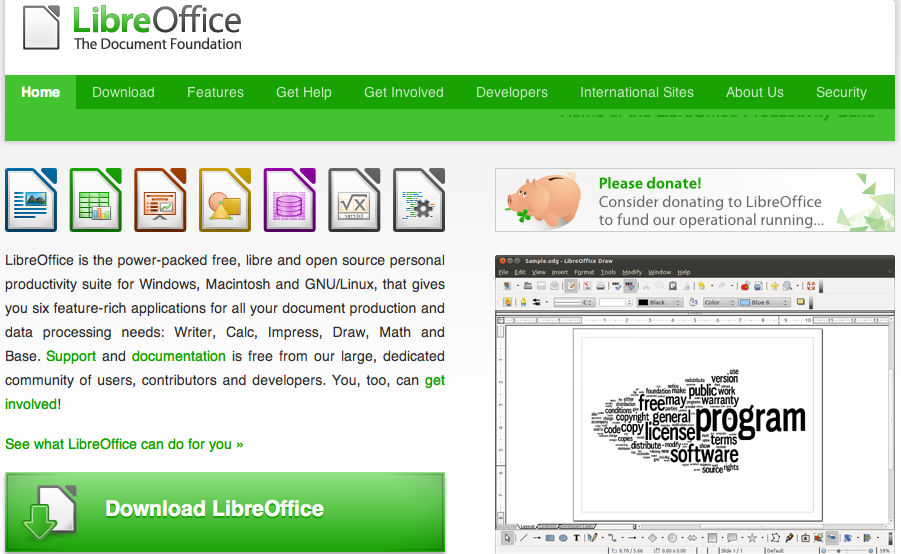
\includegraphics[width=12cm]{img/libre_web.png}
\caption{LibreOffice web site}
\end{figure}

Ubuntu is a Linux kernel based operating system. It is based on Debian Linux distribution\footnote{\url{http://www.debian.org/}}. Ubuntu is founded by the UK-based company Canonical Ltd. Unlike the other commercial vendors of Linux operating system (OS), Canonical doesn't make different "community" and "enterprise" variants of its product. This strategy has created large attraction among the users.   

\begin{figure}[H]
\centering
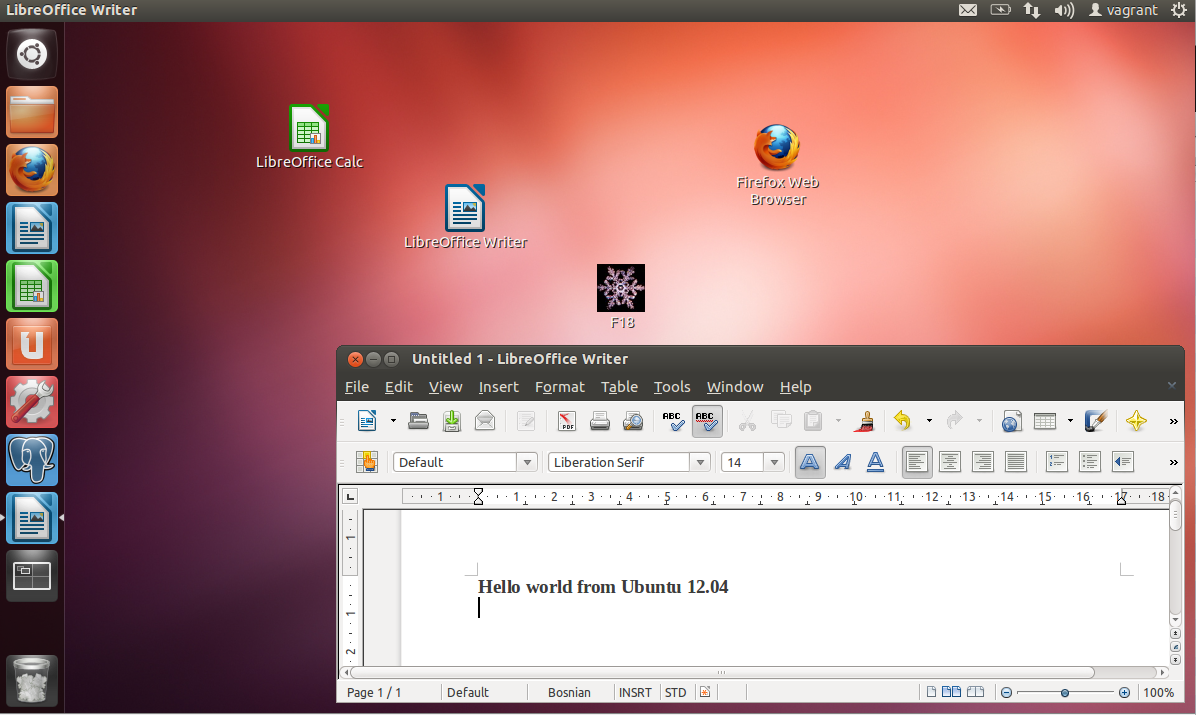
\includegraphics[width=12cm]{img/ubuntu_desktop.png}
\caption{Ubuntu desktop OS}
\end{figure}


\section{Software forking}

It is already said that the LibreOffice is the fork of OpenOffice.  A project fork happens when developers take a copy of source code from one software package and start independent development on it\footnote{\url{http://en.wikipedia.org/wiki/Fork\_(software\_development)}}. 

Free and open source software may be \textbf{legally forked} without the approval of those currently managing a software project or distributing the software, per the definitions of "free software and "open source"".

The negative implication of forking is the splitting of a development community. The right to fork is the core right for OSS user. If some group doesn't agree on the current functioning of OSS project, it has right to try on its own - it has right to fork.

LibreOffice is considered as a great example of positive effect of forking.    

\section{Piracy}

The word "piracy" is used to describe the ubiquitous, increasingly digital practices of copying that fall outside the boundaries of copyright law. The term blurs, and is often used intentionally to blur, important distinctions between types of uncompensated use. These range from the clearly illegal, such as commercial-scale, unauthorized copying for resale, to disputes over the boundaries of fair use and first sale as applied to digital goods, to the wide range of practices of personal copying that have traditionally fallen below the practical threshold of enforcement\citep{mediapiracy}

\subsection{BSA's partial way of piracy accounting}

\begin{quotation}
\emph{In 2009, more than four out of 10 software programs installed on personal computers around the world were stolen, with a commercial value of more than \$51 billion. Unauthorized software can manifest in otherwise legal businesses that buy too few software licenses, or cover criminal enterprises that sell counterfeit copies of software programs at cut-rate prices, online or offline.}

\emph{However, the impact of software piracy goes beyond revenues lost to the software industry, starving local software distributors and service providers of spending that creates jobs and generates much-needed tax revenues for governments around the world.}\citep{bsapiracyimpact}
\end{quotation}\\
This view on piracy accounting is considered partial because it doesn't take into account the positive impact of piracy on market position of top-tier (closed) vendors. As BSA\footnote{Business software alliance} and similar organizations mainly presents interests of those vendors, their point of view is understandable.  

\subsection{Software "Lock-in"}
"Lock-in" occurs when the costs of leaving a particular software environment are high - whether because switching would require significant repurchasing of software, or because the use of less common standards is disadvantageous, or simply due to costs of retraining. For near-monopolies such as Microsoft in the operating systems and office software markets, network effects reinforce market power and increase the value of their products.

Lock-in effects, in turn, ensure that customers are less likely to switch to competitors.

\subsection{Software piracy as an instrument for market dominance}  
In software markets, network effects refer to contexts in which the value of software rises with the size of the installed base. The more widely used piece of software or software service, the more it becomes a de facto standard that shapes user decisions about adoption and investment. Platform technologies such as operating systems exhibit strong network effects because a popular platform will foster a rich secondary market in applications and services, which in turn increases the platform’s value. 

As BSA piracy figures indicate, these dynamics in emerging economies are primarily a function of pirated-software adoption, not legal adoption. Piracy, in effect, has allowed the major vendors to dominate low- and middle-income markets (or, as they develop, market segments within them) that they have little financial incentive to serve. 

Perhaps most important for market-dominating firms, piracy acts as a \textbf{barrier to entry for competition, especially "free" open-source alternatives} that have no upfront licensing costs. When these emerging markets begin to grow, as most did in the last decade, piracy ensures they do so along paths shaped by the powerful network and lock-in effects associated with the market leaders.

\subsection{Software piracy full accounting}
These factors should figure in any full accounting of the \textbf{costs} and \textbf{benefits} of software piracy for top-tier vendors. Top-tier vendors have established and maintained their dominant positions in emerging markets through piracy, often prior to or in the absence of significant local investment. Any losses they incur at the margins of the consumer and business markets in those countries should be weighed against the value of maintaining their dominant positions. For near-monopolies, we would argue that this value is very high. For vendors working in highly competitive markets or selling products that do not function as standards or platforms, that value is clearly lower.\citep{mediapiracy}

\chapter{OSS in Bosnia and Herzegovina}
\vspace*{-0.7cm}
Regarding Information technology (IT) in general, BiH is underdeveloped, emerging market. It has high rate of software piracy and low rate of local software production. BiH is a great example of positive effects of software piracy for top-tier vendors. The visibility of OSS solutions and products by IT users is insignificant.
\section{Government moves}
Recent government’s moves in this field have served to the near-monopoly of position of top-tier vendors. 

"Law about fiscal systems"\footnote{\url{http://www.pufbih.ba/sr/zakon-o-fiskalnim-sistemima/pravilnici}} didn't enforce IT vendors to make technology neutral solutions. As the result we have got "Windows-only" fiscal systems on the market. Soon after the implementation of the fiscal law, the Government has begun an action on combating the software piracy. But, that action looked more like action of top-tier vendor's (Microsoft, Autodesk, etc) \textbf{private police} than Government move on enforcement of Intellectual property (IP) laws. There was no public campaign, only tax payers’ brutal money extortion. Open source software is not mentioned at all as a viable alternative to the illegal software.
\section{Monocultural IT education in BiH}
%\needspace{7\baselineskip}
OSS presence in IT education and education in general is inadequate. There is no care about vendor neutrality in IT education. OSS is not mentioned as viable alternative to the software of market leaders. The lack of adequate presentation through the education leads to low interest and lack of knowledge about OSS among young people. If this trend continues, the new generation of Bosnian IT developers and end-users is going to be IT monoculture - addicted to top-tier vendors. It can be called as \textbf{IT neo-colonialism}.

\chapter{OSS adoption in region - Slovenia} 
The article "Phenomena of Open Source and Slovenia's adoption" by Matej Mertik\footnote{Faculty of Information studies in Novo Mesto} greatly explains different standpoint of Slovenian state regarding OSS:
  
\begin{quotation}
\emph{Slovenia is still far behind in terms of open source adoption; however we have some excellent predispositions that show that there are good opportunities for Slovenia to catch up and use all the possibilities and advantages of this phenomena.}

\emph{Firstly, from a social perspective, open source software development is about collaboration and knowledge sharing, which are both on the rise in our culture.} 

\emph{Secondly, open source software eliminates a significant proportion of licence costs, which could improve the competitiveness of the small to medium sized companies that dominate in Slovenian economy.} 

\emph{Thirdly, there is an increasing acceptance of open source in the public sector through establishment of open source policies in European Union.} 

\emph{And last but not the least, while open source may not have a long history, it is set to computing in Slovenia.}\citep{oss_slovenia}
\end{quotation}

Slovenia is making strategic moves in OSS adoption. They recognize OSS as a medium for building local capacities in IT and today's economy in general. They are systematically raising OSS awareness among citizens. Education, of course, has the central role in this strategy.

They consider investment in OSS as investment in their prosperity.
 
\chapter{Conclusion}

BiH policy makers do not recognize the potential of the OSS. They suffer of classic "OSS ignorance syndrome". Today's IT world is largely built with OSS. It can be said that BiH society "lives" in the IT past\footnote{"Windows-only" era: '90-ties of the last century}.  

Slovenia's example clearly shows that open source software is not just an alternative to closed source counterparts. There is clear public interest to promote and invest into it. 

At the end, OSS is all about knowledge. As we live in ``Information Age''\footnote{\url{http://en.wikipedia.org/wiki/Information\_Age}}, OSS adoption is the question of basic \textbf{competitiveness} in today's world. 

% -------------------------------------------------
\bibliography{literatura}
\bibliographystyle{fit}

% -------------------------------------------------
\appendix

\chapter{Software toolset}
\begin{enumerate}
  \item Mac OS X 10.6.8
  \item mvim, vim tekst editor ver 7.3
  \item MacTex - pdfTeX 3.1415926-2.3-1.40.12 (TeX Live 2011)
\end{enumerate}

\chapter{Notes}

\begin{itemize}
  \item Document source code \url{https://github.com/hernad/FIT\_ENG/blob/master/seminarski/OS\_BiH.tex}
  \item Document in PDF format \url{https://github.com/hernad/FIT\_ENG/raw/master/seminarski/OSS\_BiH.pdf}
  \item redmine ticket - "Engleski jezik seminarski: rad OSS u BiH" \url{http://redmine.bring.out.ba/issues/28517}

\end{itemize}

\end{document}
